\documentclass[journal,12pt,twocolumn]{IEEEtran}
\usepackage{graphicx}
\graphicspath{{./figs/}}{}
\usepackage{amsmath,amssymb,amsfonts,amsthm}
\newcommand{\myvec}[1]{\ensuremath{\begin{pmatrix}#1\end{pmatrix}}}
\usepackage{listings}
\usepackage{watermark}
\usepackage{titlesec}
\let\vec\mathbf

\titlespacing{\subsection}{0pt}{\parskip}{-3pt}
\titlespacing{\subsubsection}{0pt}{\parskip}{-\parskip}
\titlespacing{\paragraph}{0pt}{\parskip}{\parskip}
\newcommand{\figuremacro}[5]{
    
}
\lstset{
frame=single, 
breaklines=true,
columns=fullflexible
}
\thiswatermark{\centering \put(0,-105.0){
\includegraphics[scale=0.05]{iitlogo.jpg}} }

\sloppy
\title{\mytitle}
\title{
Conic Assignment 
}
\author{T.Siva Parvathi(FWC22089)}
\begin{document}
\maketitle
\tableofcontents
\bigskip


\section{\textbf{problem}}
Q.The locus of the mid-point of the lines segment joining the focus to a moving point on the parabola $y^2$=4a$x$ is another parabola with directrix

\section{\textbf{solution}}
The standard conic equation is,\\
\begin{align}
\label{eq:one}
\vec{x}^\top\vec{Vx}+2\vec{u}^\top\vec{x}+f=0
\end{align} 
 where,
$\vec{V}=\myvec{0&0 \\0&1}$\\ $\vec{u}=\myvec{-2a\\0}$ and $f=0$ \\


\begin{figure}[h]
    \centering
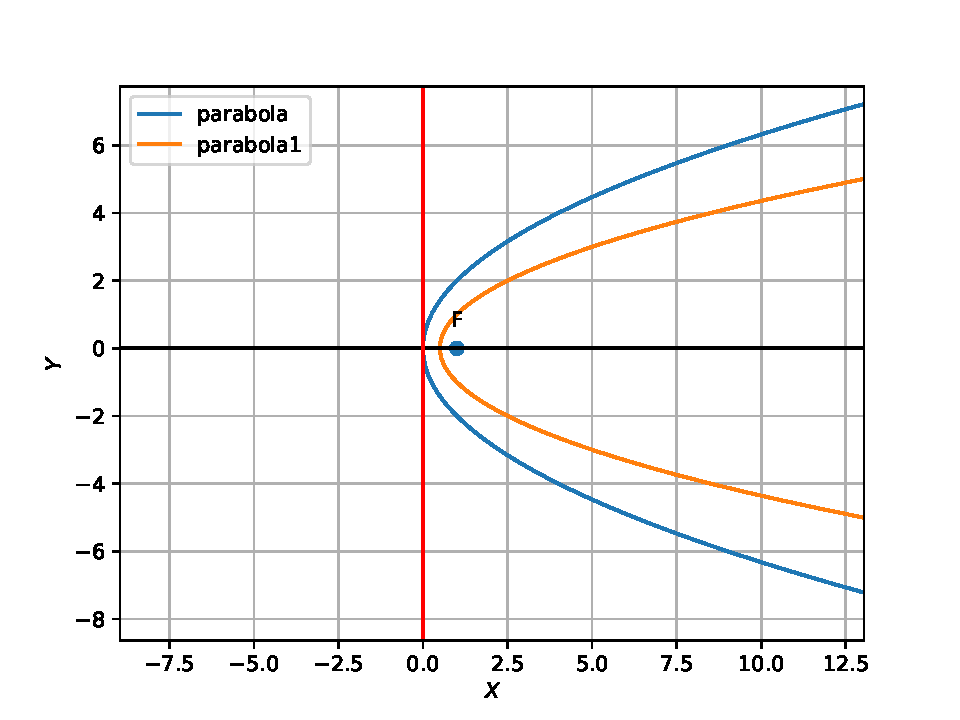
\includegraphics[width=\columnwidth]{cofig.pdf}
\caption{Labeling locus parabola with directrix for a given parabola}
    \label{fig:my_label}
\end{figure}


For the standard conic,\\
\begin{align}
\label{eq:two}
\vec{u}=\frac{\eta}{2}e_1 , e=1
\end{align}
where, $e_1=\myvec{1\\0}$
equating values of u,\\
\begin{center}
$\frac{\eta}{2}\myvec{1\\0}=\myvec{-2a\\0}$\\
$\myvec{\frac{\eta}{2} \\ 0}=\myvec{-2a\\0}$\\
$\frac{\eta}{2}e_1=-2a$\\
$\eta=-4a$
\end{center}
\section{\textbf{figure}}
Foci of the standard parabola is given by,\\
\begin{align}
\label{eq:three}
\vec{F}=\frac{-\eta}{4\lambda_2}e_1 , e=1
\end{align} 
By substituting $\eta$ value we get,\\
\begin{center}
$\vec{F}=-\frac{-4a}{4}\myvec{1\\0}$\\
$\vec{F}=\myvec{a\\0}$
\end{center}
let moving point on the parabola be 'q',then the equation is,
\begin{align}
\label{eq:four}
\vec{q}^\top\vec{Vq}+2\vec{u}^\top\vec{q}+f=0
\end{align}
the mid-point when line segment joining the focus to moving point on the parabola be 'h'.
\begin{align}
\label{eq:five}
\vec{h}=\frac{\vec{q+F}}{2}
\end{align}
\begin{align}
\label{eq:six}
\vec{q}=2\vec{h}-\vec{F}
\end{align}
Substitute \eqref{eq:six} in \eqref{eq:four}\\
\begin{align}
\label{eq:seven}
(2\vec{h}-\vec{F})^\top\vec{V}(2\vec{h}-\vec{F})+2\vec{u}^\top(2\vec{h}-\vec{F})+f=0
\end{align}
%$(2\vec{h}$-$\myvec{a\\0})^\top\myvec{0&0\\0&1}(2\vec{h}$-$\myvec{a\\0})+2\myvec{-2a&0}(2\vec{h}$-$\myvec{a\\0})+0=0$\\
$4\vec{h}^\top\vec{Vh}-\vec{F}^\top\vec{VF}-2\vec{h}^\top\vec{VF}-2\vec{F}^\top\vec{Vh}+4\vec{u}^\top\vec{h}-2\vec{u}^\top\vec{F}+f=0$\\
By solving we get the new parabola equation,\\
\begin{align}
\label{eq:ei}
y^2-2ax+a^2=0
\end{align}
from above the locus parabola equation can be written as, \\
\begin{align}
\label{eq:ni}
\vec{h}^\top\vec{V}_{1}\vec{h}+2\vec{u}_{1}^\top\vec{h}+f_1=0
\end{align} 
where,
$\vec{V}_{1}=\myvec{0&0 \\0&1}$\\ $\vec{u}_{1}=\myvec{-a\\0}$ and $f_1=a^2$ \\
The new parabola equation in terms of old parabola equation is,\\
\begin{center}
$\vec{x}^\top\vec{V}\vec{x}+\vec{u}^\top\vec{x}+(f+d)=0$
\end{center}
The directrix of a conic is given by,
\begin{align}
\label{eq:te}
\vec{n}^\top\vec{x}=c
\end{align}
The directrices of \eqref{eq:ni} is given by,\\
\begin{align}
\label{eq:ele}
\vec{n}=\sqrt{\lambda_2}\vec{p}_{1}
\end{align}
\begin{align}
\label{eq:t}
c=\frac{\|\vec{u}\|^2-\lambda_2 f}{2\vec{u}^\top\vec{n}} , e=1
\end{align}
where the eigen values and eigen vectors are,\\
\begin{align}
\label{eq:twe}
\lambda_1=0 , \lambda_2=1\\
\vec{p}_{1}=\myvec{1\\0}, \vec{p}_{2}=\myvec{0\\1} 
\end{align}
substituting values in \eqref{eq:ele} we get,\\
\begin{align}
\label{eq:thir}
\vec{n}=\myvec{1\\0}
\end{align}
substituting values in \eqref{eq:t},\\
$c=\frac{a^2-a^2}{2\myvec{-a & 0}\myvec{1\\0}}$\\
\begin{align}
\label{eq:fourteen}
c=0
\end{align}
put n and c in directrix equation we get,
\begin{align}
\label{eq:fif}
\myvec{1&0}\vec{x}=0
\end{align}
        Therefore,the locus of the mid-point of the lines segment joining the focus to a moving point on the parabola $y^2$-$4ax=0$ is another parabola $y^2$-$2ax$+$a^2=0$ with directrix $x=0$.\\



\section{\textbf{software}}
\begin{lstlisting}
https://github.com/sivaparvathi-tungala/fwc_module_1/tree/main/conic
\end{lstlisting}

\end{document}